\documentclass[UTF8,a4paper,10pt,nocolorlinks]{ctexart}
\usepackage[left=2.50cm, right=2.50cm, top=2.50cm, bottom=2.50cm]{geometry} %页边距
\CTEXsetup[format={\Large\bfseries}]{section} %设置章标题居左   
\usepackage{ctex}
\CTEXoptions[today=old]
\usepackage{cite}
% 代码块儿
\usepackage{textcomp} % 必须加上,否则报错
\usepackage{listings}
\usepackage{xcolor}
% \usepackage{fontspec}
% \setmonofont{Consolas}
\usepackage{varioref}       % ref 跨页调用
\usepackage{ctex}
\usepackage{multicol}
\usepackage{amssymb}        % 等于号 上面 加一个三角形
\usepackage{setspace}
\usepackage{tikz} % package used for the tikz
\usepackage{mdframed}
\usepackage{titletoc}
\usepackage{etoolbox}

\usepackage{helvet}
\usepackage{caption}
\usepackage{multicol} %用于实现在同一页中实现不同的分栏
\usepackage{changepage}
\usepackage{graphics}
\usepackage{amsmath, amsfonts, amssymb} % math equations, symbols
\usepackage[english]{babel}
\usepackage{color}      % color content 设置字体颜色
\usepackage{graphicx}   % import figures
\usepackage{url}        % hyperlinks
\usepackage{bm}         % bold type for equations
\usepackage{multirow}
\usepackage{booktabs}
\usepackage{epstopdf}
\usepackage{epsfig}
\usepackage{algorithm}
\usepackage{algorithmic}
\usepackage[pagestyles]{titlesec}
% \renewcommand{\algorithmicrequire}{ \textbf{Input:}}     % use Input in the format of Algorithm  
% \renewcommand{\algorithmicinput}{ \textbf{Input:}}     % use Input in the format of Algorithm  
\renewcommand{\algorithmicensure}{ \textbf{Input:}} % use Initialize in the format of Algorithm  
% \renewcommand{\algorithmicreturn}{ \textbf{Output:}}     % use Output in the format of Algorithm  
\renewcommand{\figurename}{图}
% 引用参考文献标号显示在右上角
\newcommand{\upcite}[1]{\textsuperscript{\textsuperscript{\cite{#1}}}}

\newpagestyle{teststyle}{
  \sethead{学号: 2019520941}{\sectiontitle}{第\thepage页}
  \renewcommand{\makeheadrule}{
    \makebox[0pt][l]{\rule[-.3\baselineskip]{\linewidth}{.5pt}}
    \rule[-.4\baselineskip]{\linewidth}{.5pt}
  }
}
\usepackage{color}
\usepackage{subfigure}
\usepackage{changepage}
\usepackage{fancyhdr} %设置页眉、页脚
\pagestyle{fancy}  %%%单线页眉
\fancyhead{}
\fancyhead[LO]{chapter 4 notebook}
\fancyhead[RO]{fengxuewei}
% \fancyfoot[RO]{\thepage}
\fancypagestyle{plain}{%
  \pagestyle{fancy}
}
\usepackage{shorttoc}
\usepackage{xcolor}
\usepackage{mdframed}
\usepackage{titletoc}
% \renewcommand{\today}{\CJKnumber\year 年 \CJKnumber\month 月 \CJKnumber\day 日}

\DeclareRobustCommand{\chuhao}{\fontsize{42pt}{\baselineskip}\selectfont}  % 初号
\DeclareRobustCommand{\xiaochu}{\fontsize{36pt}{\baselineskip}\selectfont} % 小初
\DeclareRobustCommand{\yihao}{\fontsize{26pt}{\baselineskip}\selectfont}   % 一号
\DeclareRobustCommand{\xiaoyi}{\fontsize{24pt}{\baselineskip}\selectfont}  % 小一
\DeclareRobustCommand{\erhao}{\fontsize{22pt}{\baselineskip}\selectfont}   % 二号
\DeclareRobustCommand{\xiaoer}{\fontsize{18pt}{\baselineskip}\selectfont}  % 小二
\DeclareRobustCommand{\sanhao}{\fontsize{16pt}{\baselineskip}\selectfont}  % 三号 
\DeclareRobustCommand{\xiaosan}{\fontsize{15pt}{\baselineskip}\selectfont} % 小三
\DeclareRobustCommand{\sihao}{\fontsize{14pt}{\baselineskip}\selectfont}   % 四号
\DeclareRobustCommand{\xiaosi}{\fontsize{12pt}{\baselineskip}\selectfont}  % 小四
\DeclareRobustCommand{\wuhao}{\fontsize{10.5pt}{\baselineskip}\selectfont} % 五号
\DeclareRobustCommand{\xiaowu}{\fontsize{9pt}{\baselineskip}\selectfont}   % 小五
\DeclareRobustCommand{\liuhao}{\fontsize{7.5pt}{\baselineskip}\selectfont} % 六号
\DeclareRobustCommand{\xiaoliu}{\fontsize{6.5pt}{\baselineskip}\selectfont}% 小六
\DeclareRobustCommand{\qihao}{\fontsize{5.5pt}{\baselineskip}\selectfont}  % 七号

\lstset{numbers=left,numberstyle=\tiny,
breaklines=true,  %代码过长则换行
keywordstyle=\color{blue!70},commentstyle=\color{red!50!green!50!blue!50},frame=shadowbox, rulesepcolor=\color{gray!20!green!20!blue!20},escapeinside=``,xleftmargin=2em,xrightmargin=2em, aboveskip=1em}

\providecommand{\keywords}[1]{\textbf{\textit{keywords---}} #1}

 
\usepackage{hyperref} %bookmarks
% \usepackage[colorlinks,linkcolor=red,anchorcolor=blue,citecolor=green,CJKbookmarks=True]{hyperref}
\hypersetup{colorlinks, bookmarks, unicode} % unicode
 
\captionsetup[figure]{labelfont={bf},labelformat={default},labelsep=period,name={图}}
\newenvironment{figurehere}
{\def\@captype{figure}}
{}
 
% \title{\textbf{A*算法和模拟退火算法无人机领域的应用}}
% \author{ 冯学伟 \thanks{学号:2019520941}}
% \date{\today}

%标题、作者及日期
% \huge{\textbf{无人机导航控制}}\\[3mm]
% \Large{\textbf{The Navigational Control In The Field Of Unmanned Air Vehicle}}\\[1mm]

\title{chapter 4. Forces and Moments 力和力矩}
\author{冯学伟}
\date{\today}

\begin{document}
    \maketitle
    \begin{itemize}
      \item 目标: 描述作用在 无人机上的力和力矩, 
      \item 来源: 重力($f_{g}$), 空气动力学($f_{a}, m_{a}$), 推力($f_{p}, m_{p}$) (f 是力, m 是动量) 见公式组\ref{equ:1}
      \item 推导的表达式: 上面的每个力和力矩的表达式
      \item 第一节: 重力
      \item 第二节: 空气动力和力矩
      \item 第三节: 推力的力和力矩
      \item 第四节: 大气的扰动 被建模为风速的变化,并通过空气动力和扭矩推导出运动方程
    \end{itemize}
    
    \begin{align}
      f &= f_{g} + f_{a} + f_{p}  \nonumber\\
      m &= m_{a} + m_{p}
      \label{equ:1}
    \end{align}
    其中的 f 是作用在 飞行器上面的合力, m 是作用在飞行器上面的总力矩.
    
    \section{力矩}
    \begin{figure}[htpb]
      \centering
      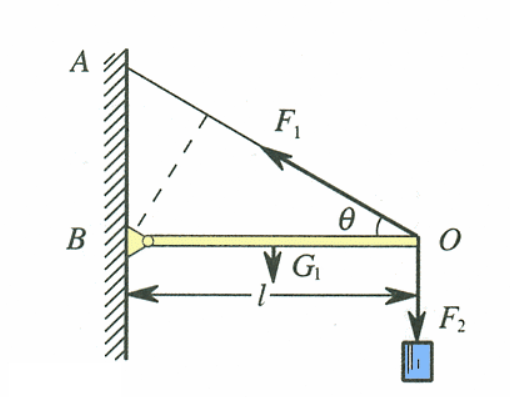
\includegraphics[width=0.8\textwidth]{picture/moment.png} % 不能保存 gif 格式的图片
      \caption{力矩示意图}
      \label{fig_moment}
    \end{figure}
    力矩表示力对物体作用时所产生的转动效应的物理量. 力对某一点的力矩的大小为该点到力的作用线所引垂线的长度(即力臂)乘以力的大小,其方向则垂直于垂线和力所构成的平面用右手螺旋法则来确定\ref{fig_moment}
    \section{量纲式}
    将一个物理导出量用若干个基本量的乘方之积表示出来的表达式,称为该物理量的量纲式,简称量纲。 
    它是在选定了单位制之后,由基本物理量单位表达的式子。
    有量纲的物理量都可以进行无量纲化处理。

    线应变表示为线长度的增量除以初始长度,由于分子、分母的量纲均为长度单位m,故线应变是一个无量纲物理量。无量纲按照个人理解应该是 单位为1. 
    即无量纲的物理量其单位在计算时一般取为数字1.
    \section{雷诺数和马赫数}
    \subsection{雷诺数}
    雷诺数(Reynolds number)一种可用来表征流体流动情况的无量纲数。
    \textcolor{red}{$Re = \frac{\rho vd}{\mu}$},其中$v, \rho, \mu$分别为流体的流速、密度与黏性系数,$d$为一特征长度。
    \par 例如流体流过圆形管道,则d为管道的当量直径。利用雷诺数可区分流体的流动是层流或湍流,
    也可用来确定物体在流体中流动所受到的阻力。

    \subsection{马赫数}
    流体力学中表征流体可压缩程度的一个重要的无量纲参数,记为Ma,
    定义为流场中某点的速度v同该点的当地声速c之比,即\textcolor{red}{$Ma= \frac{v}{c}$}, 它是以奥地利科学家E.马赫的姓氏命名的。

    \section{Gravitational Forces 重力}
    作用在无人机上的地球的重力场和物体的质量大小成比例, 方向是指向$k^{i}$ 并且与无人机的质量和重力加速度$g$的乘积(by)成比例. \par
    在 vehicle frame $F^{v}$ , 重力作用在质量的中心, 公式见: \ref{equ:2}.

    
    \begin{gather} % 输入多行公式
      f_{g}^{v} = \begin{pmatrix} 
        0 \\
        0 \\
        mg \\
      \end{pmatrix}
      \label{equ:2}
    \end{gather}

    在第3章中应用牛顿第二定律时,我们沿 body frame 的轴进行求和, 因此我们需要将重力转换到 body frame 下, 转换公式如: \ref{fig:equ_1};

    因为重力穿过在物体的质心, 所以没有力矩产生. 
    \begin{figure}[htpb]
      \centering
      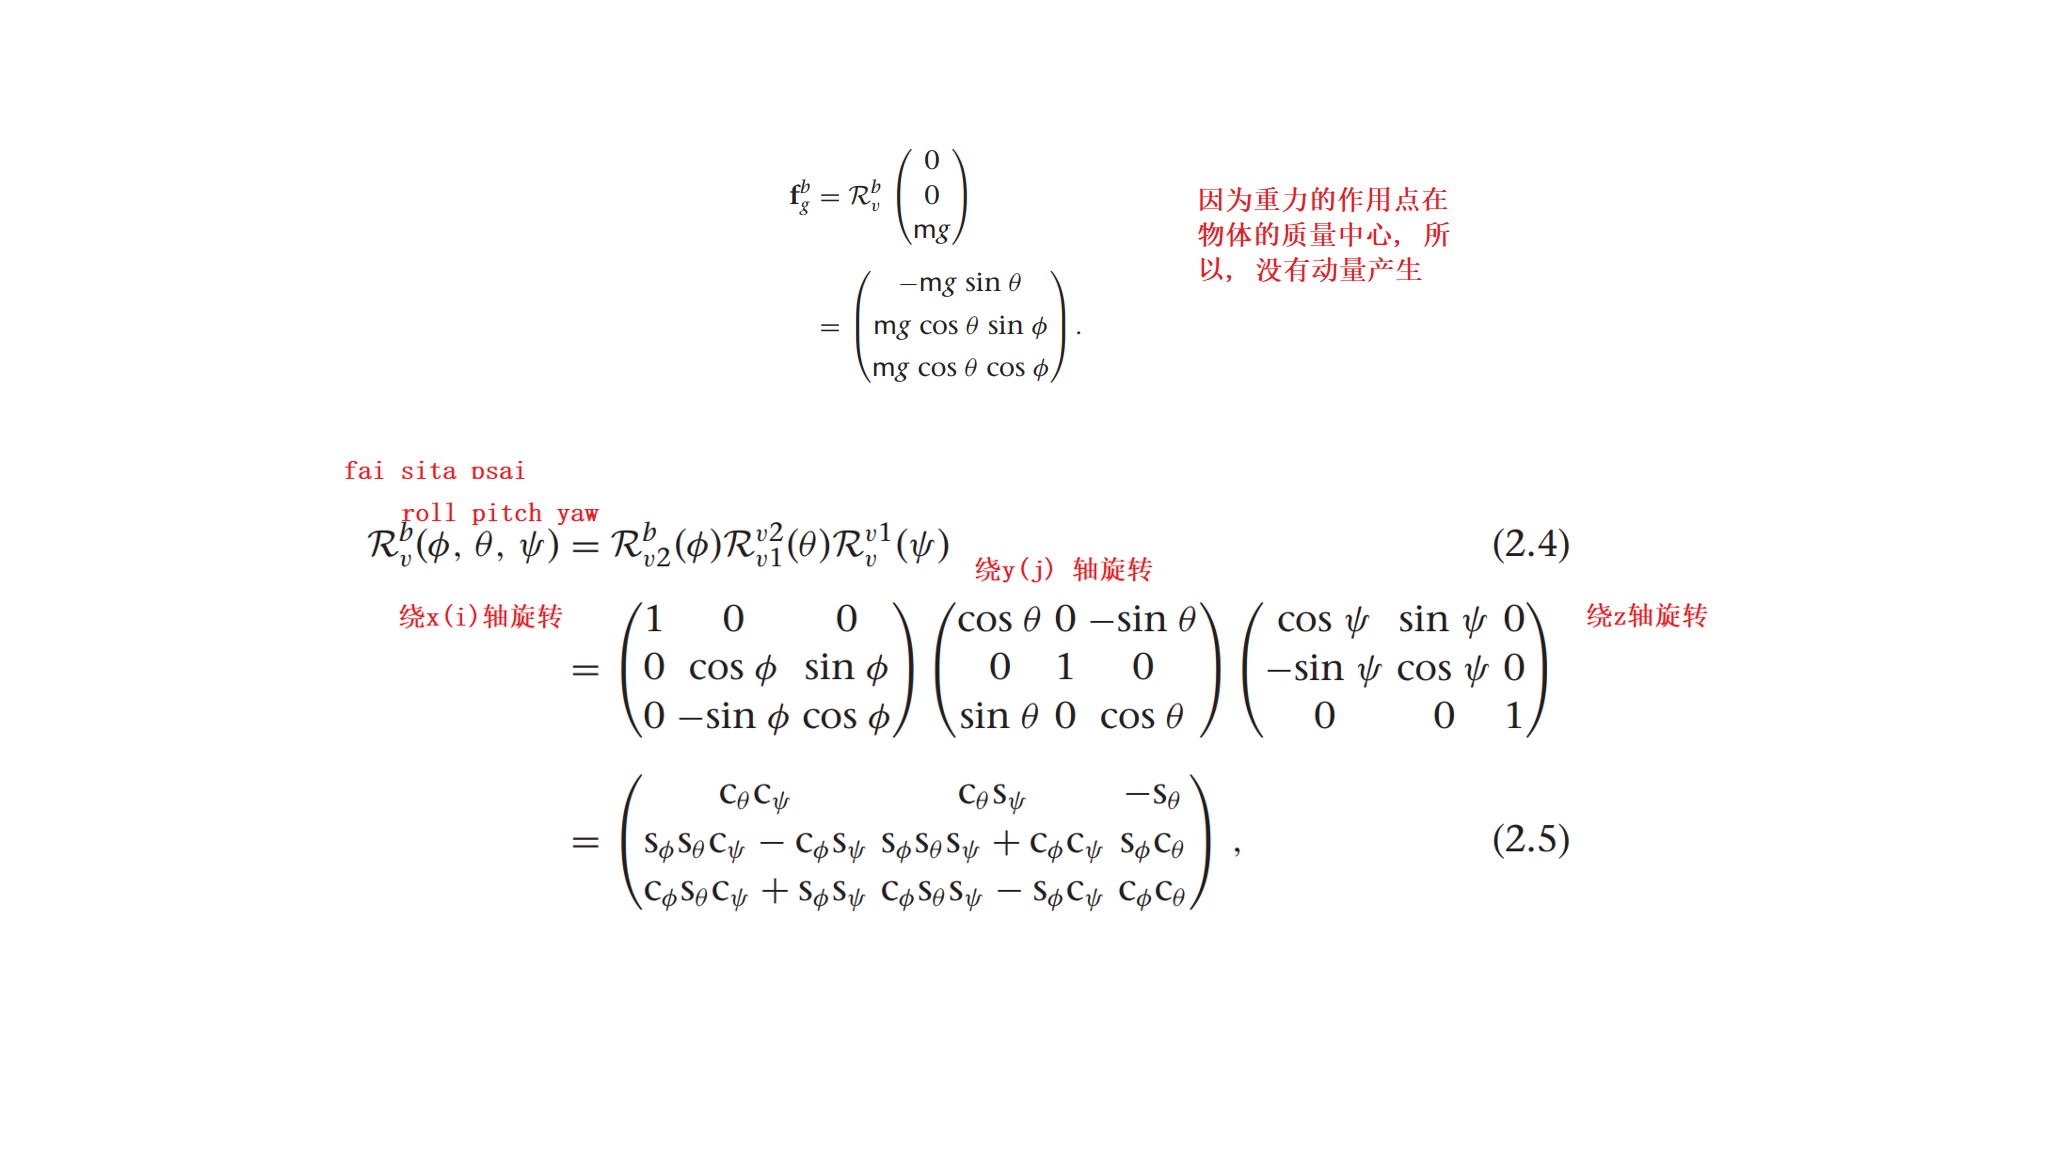
\includegraphics[width=0.8\textwidth]{picture/4_equ_1.png}
      \caption{重力转换公式}
      \label{fig:equ_1}
    \end{figure}

    \section{空气动力学和动量}
    当无人机在空中飞行时, 会在无人机附近产生空气流动 形成一定的压力 pressure, 

    \begin{figure}[htpb]
      \centering
      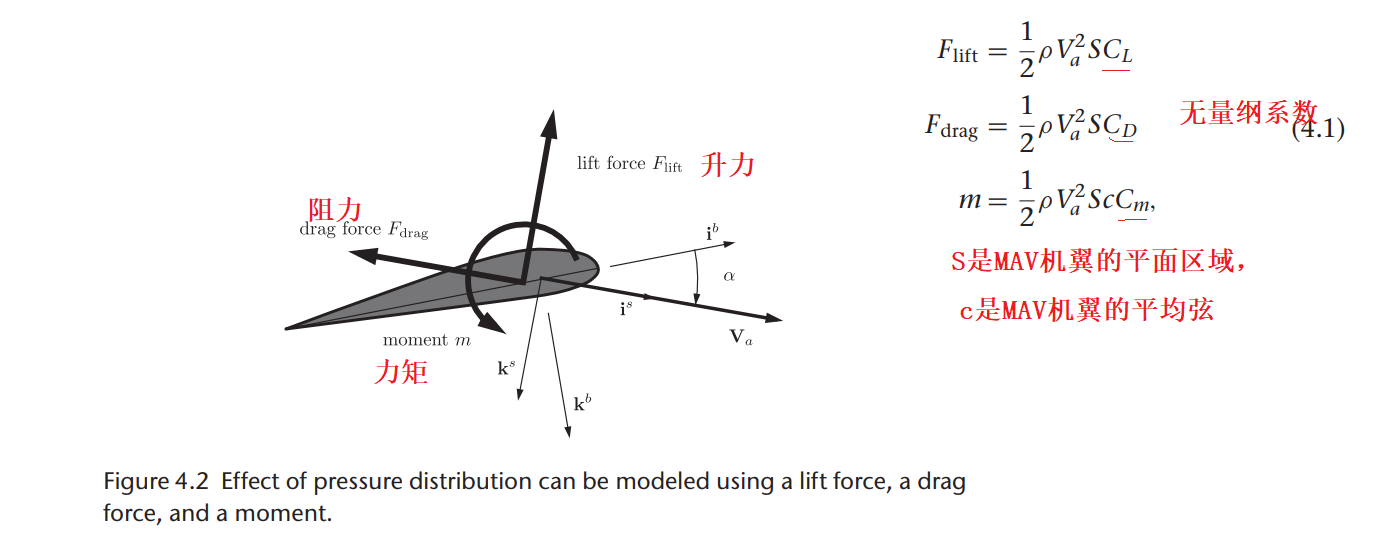
\includegraphics[width=0.8\textwidth]{picture/4_equ_2.png}
      \caption{空气动力几何模型}
      \label{fig:equ_2}
    \end{figure}

    见图\ref{fig:equ_2}, $C_{L}$, $C_{D}$, 和 $C_{m}$都是非量纲系数, $S$是无人机机翼的平面区域, $c$是MAV机翼的平均弦
    \par
    升力, 阻力, 和 pitch 力矩系数受机翼的形状 雷诺数 马赫数和迎角的影响, 其中, 雷诺数和马赫数的影响大约是常量; 
    \textcolor{red}{因此我们考虑的是角度$\alpha, \beta$, 以及角速率 $p, q, r$ 和 控制平面在空气动力学系数上的偏差.} \par
    \begin{itemize}
      \item 一般将空气动力学的力和力矩分为两组: 纵向和横向;
      \item 纵向的力和力矩作用在 $i^{b}-k^{b}$ 平面(也称为pitch平面), 包含了在$i^{b}$和$k^{b}$两个方向上的力(升力和阻力), 在$j^{b}$轴上的是力矩;
      \item 横向的力和力矩包括$j^{b}$方向上的力和 $i^{b}$和$k^b$上的力矩.
    \end{itemize}  

    \subsection{control Surfaces 控制平面}
    在描述由于升平面产生的空气动力和力矩之前, 我们需要定义操作无人机的控制平面. \par
    控制平面常常被用来修改空气动力和力矩. 对于标准无人机初始结构, 控制平面包含了升降舵, 副翼和方向舵(
    the elevator, the aileron, and the rudder), 见\ref{fig:confi}. 其他的平面比如扰流板,襟翼和前翼(spoilers, flaps, and
    canards) 不会讨论, 但是建动力学模型的方法都是类似的.

    \begin{figure}
      \centering
      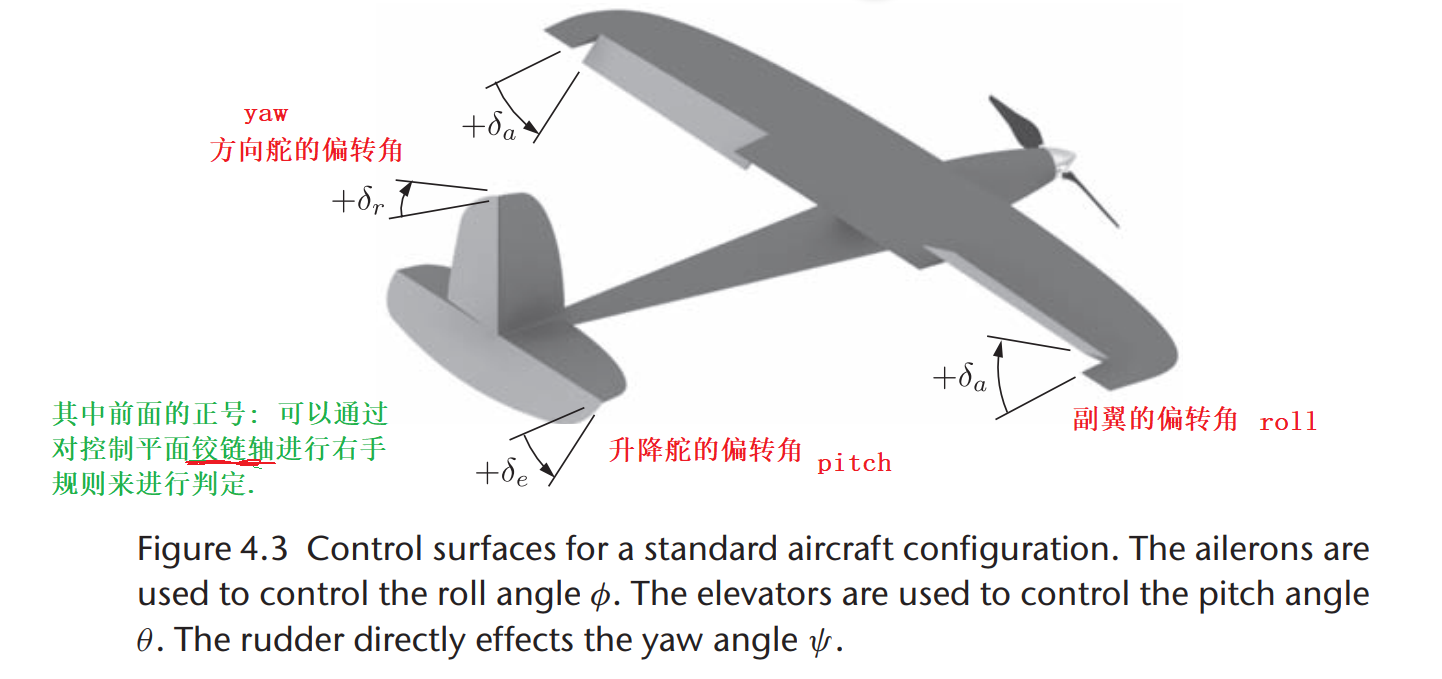
\includegraphics[width=0.8\textwidth]{picture/standard_confi.png}
      \caption{方向舵-升降舵初始结构}
      \label{fig:confi} % scale=0.3 将图片等比例缩小3倍  
    \end{figure}
    \begin{figure}[htpb]
      \centering
      \subfigure[ruddervators configuration]{
        \label{fig:vtail} 
        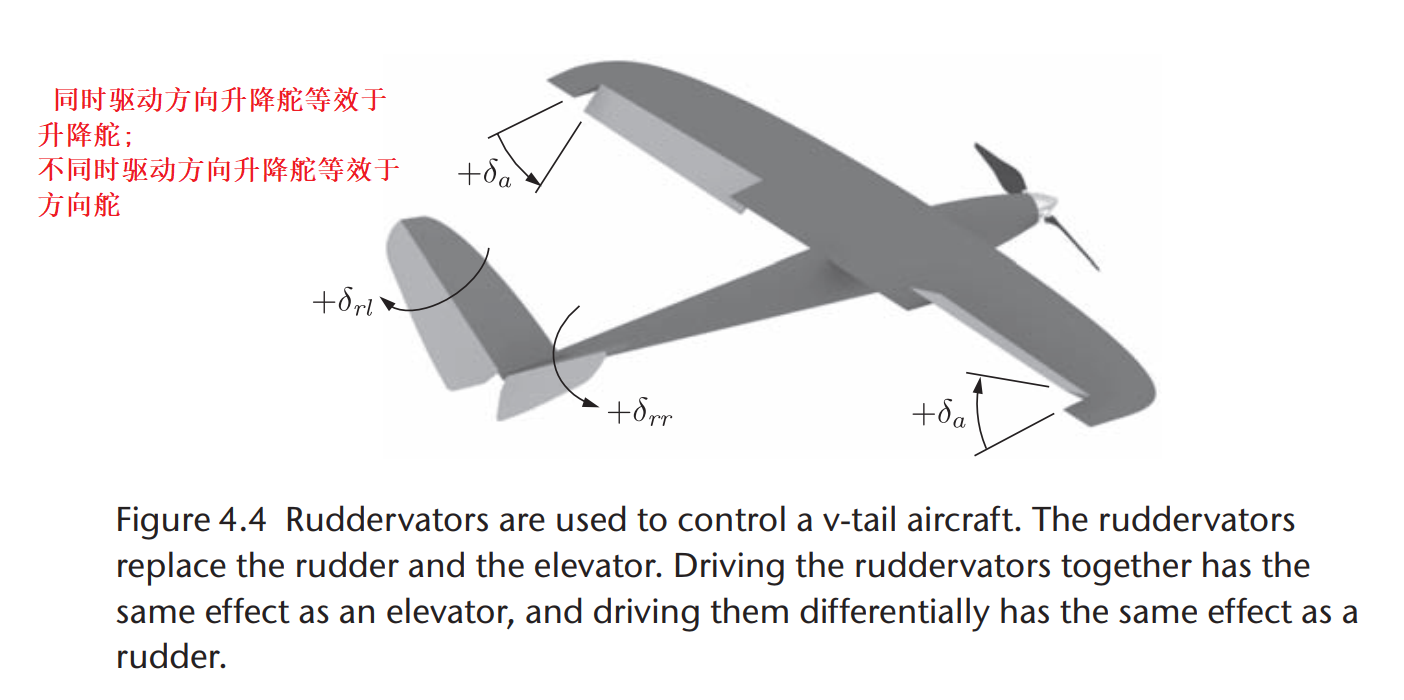
\includegraphics[scale=0.3]{picture/vtail_confi.png}}
      \hspace{0.5in} % 两图片之间的距离
      \subfigure[elevons configuration]{
        \label{fig:elevons}
        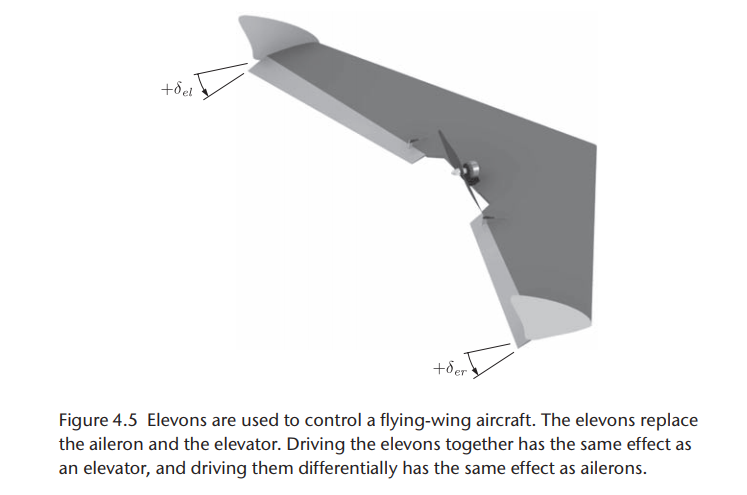
\includegraphics[scale=0.4]{picture/elevons_confi.png}}
      \caption{两种无人机初始结构分布}
    \end{figure}

    \par 在图\ref{fig:confi}中, 副翼被用来控制roll($\phi$), 升降舵控制pitch($\theta$), 方向舵被用来控制yaw($\psi$). 其中偏转角前面的 $+$ 号可以通过对控制平面铰链轴进行右手准则来决定. 
    \begin{itemize}
      \item 升降舵的铰链轴和body frame的 $j^{b}$, 对$j^{b}$轴应用右手准则表明了正向偏转代表了尾翼边缘下降. 
      \item 升降舵正向偏转: 代表了尾翼边缘下降. 
      \item 方向舵正向偏转: 代表了尾翼边缘左打. 
      \item 副翼正向偏转: 代表了两个副翼效果叠加均值为+.  
    \end{itemize}
    同时, 副翼的偏转 $\delta_{a} = \frac{1}{2} (\delta_{a-left} - \delta_{a-right})$ 的复合变形, 所以正向$\delta_{a}$代表了左翼朝下, 右翼朝上. 

    \par 
    \par 对于小型的无人机, 有两个标准初始结构 \par
    \begin{itemize}
      \item 第一种是: V字形尾翼, 见 \ref{fig:vtail} \\
      方向升降舵代替了升降舵和方向舵, 同时驱动方向升降舵效果等同于升降舵(在$j^{b}$轴上面产生一个扭力), 不同时驱动效果等同于方向舵(在$k^{b}$轴上面产生一个扭力). $\delta_{rr}$: 右方向舵角度偏转; $\delta_{rl}$: 左方向舵角度偏转. 
      数学上, 我们利用两种情形进行一个转换. 见\ref{equ:3}. 
      \par
      \textcolor{red}{相同代表了V翼两侧产生力的方向是一样的. 就会产生升降的效果; 不同的话, V翼两侧产生力的方向不一样, 通过偏转角度的不同, 从而产生力的大小不同, 合力朝着某一个方向, 这个时候,飞机会绕着$k^{b}$轴进行旋转, 机头偏向另外的一侧.}
      \begin{gather}
        \begin{pmatrix}
          \delta_{e} \\
          \delta_{r} \\
        \end{pmatrix} = 
        \begin{pmatrix}
          1 & 1 \\
          -1 & 1 \\
        \end{pmatrix} 
        \begin{pmatrix}
          \delta_{rr} \\
          \delta_{rl}
        \end{pmatrix}
        \label{equ:3}
      \end{gather}
      我们可以使用\ref{equ:3}关系, v-tail无人机的力和扭矩的关系式可以就标准的方向舵和升降舵表示出来.
      \item 另外的一种标准飞机结构, 见 \ref{fig:elevons} 升降副翼结构 \\
      $\delta_{er}$: 右升降翼舵角度偏转; $\delta_{el}$: 左升降翼舵角度偏转. \\
      同时操作两个elevons机翼效果等同于升降舵, 产生一个 $j^{b}$ 方向的扭矩. \\
      不同时操作两个elevons机翼效果等同于副翼, 产生一个 $i^{b}$ 方向的扭矩. \\
      \begin{gather}
        \begin{pmatrix}
          \delta_{e} \\
          \delta_{r} \\
        \end{pmatrix} = 
        \begin{pmatrix}
          1 & 1 \\
          -1 & 1 \\
        \end{pmatrix} 
        \begin{pmatrix}
          \delta_{er} \\
          \delta_{el}
        \end{pmatrix}
        \label{equ:4}
      \end{gather}
      
      \begin{figure}
        \centering
        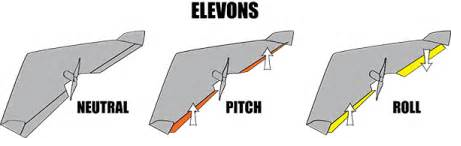
\includegraphics[width=0.8\textwidth]{picture/OIP.png}
        \caption{elevons操作效果图}
      \end{figure}

      OIP.jfif

      我们可以利用 \ref{equ:4} 来对elevons和\ref{fig:confi}进行转换. 
      故使用\ref{equ:4}关系, elevons无人机的力和扭矩的关系式可以就标准的方向舵和升降舵表示出来.
    \end{itemize}

    \subsection{纵向空气动力学}
    纵向空气动力学 导致飞机在 $i^{b}, k^{b}$ 平面(也称为pitch平面)内的移动, 
    它们是我们可能最熟悉的空气动力和力矩:升力,阻力和俯仰力矩。
    \par
    升力和阻力与稳定坐标系的轴对齐, 见\ref{fig:equ_2}(stability frame 见 \ref{fig:stable})
    \begin{figure}
      \centering
      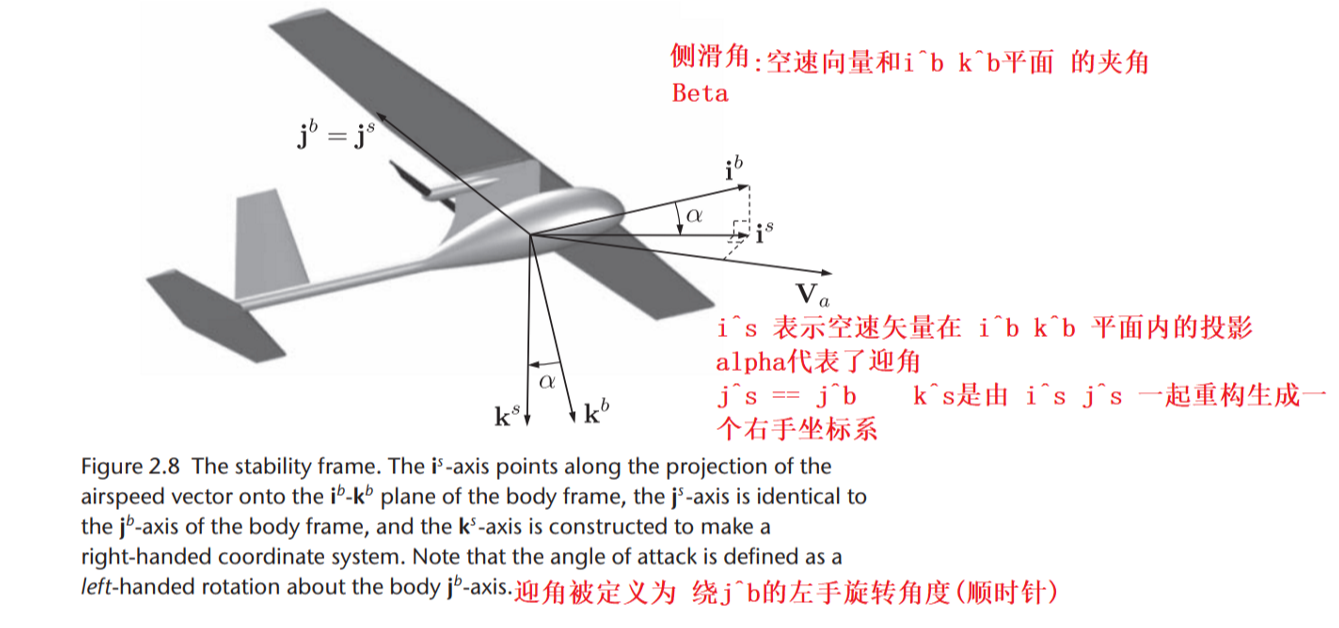
\includegraphics[width=0.8\textwidth]{picture/stability_frame.png}
      \caption{stability frame}
      \label{fig:stable}
    \end{figure}
    当表示为一个向量的时候, pitching的力矩是和 $j^{s}$ 轴对齐, 升力和阻力以及pitching力矩受迎角的影响较大, 同时, pitch角的变换率$q$和升降舵偏转角$\delta_{e}$会影响纵向力和力矩. \par
    基于这个, 我们重写了升力, 阻力和pitching力矩的表达式, 这个表达式依赖于 $\alpha, q, \delta_{e}$, 分别是迎角, pitch的变换率, 升降舵的偏转角. 
    \begin{equation}
      \begin{split}
      F_{lift} &= \frac{1}{2} \rho V_{a}^{2}SC_{L}(\alpha, q, \delta_{e}) \\
      F_{Drag} &= \frac{1}{2} \rho V_{a}^{2}SC_{D}(\alpha, q, \delta_{e}) \\
      m &= \frac{1}{2} \rho V_{a}^{2}S_{c}C_{m}(\alpha, q, \delta_{e}) \\
      \label{equ:lift_drag_moment}
    \end{split}
  \end{equation}
  一般而言: 这些力和力矩都是非线性的, 然而对于\textcolor{red}{小的迎角}, 机翼上的气流将保持层流状态, 
  在这种情形下, 升力和阻力以及pitching力矩可以\textcolor{blue}{使用线性近似可接受的精度建模}. 
  以升力表达式\ref{equ:lift_drag_moment}为例, 对其进行一个泰勒展开变形. 可得下面的式子\ref{equ:taylor_lift}.通常对这种线性近似的偏导数进行无量纲化处理.
  \begin{align}
    F_{lift} &= \frac{1}{2} \rho V_{a}^{2} S \left[ C_{L0} + \frac{\partial C_{L}}{\partial \alpha} \alpha +  \frac{\partial C_{L}}{\partial q} q + \frac{\partial C_{L}}{\partial \delta_{e}} \delta_{e} \right] \\
    C_{L0} &= constant, (\alpha = q = \delta_{e} = 0), nondimensional
    \label{equ:taylor_lift}
  \end{align}
  \textcolor{red}{$C_{L}, \alpha, \delta_{e}$ 都是无量纲数, 且$\delta_{e}$表示的是弧度, 故要对其进行无量纲化处理, 我们只需要将 $ \frac{\partial C_{L}}{\partial q} q$ 进行无量纲化处理即可}. 
  $q$的单位是 $rad$ / $s$,将 $q$ 转换为 $\frac{qc}{2V_{a}}$. 
  
  \begin{equation}
    F_{lift} = \frac{1}{2} \rho V_{a}^{2} S \left[ C_{L0} + \frac{\partial C_{L}}{\partial \alpha} \alpha +  \frac{\partial C_{L}}{\partial \frac{qc}{2 V_{a}}} \frac{c}{2 V_{a}}q + \frac{\partial C_{L}}{\partial \delta_{e}} \delta_{e} \right] 
  \end{equation}
  
  $\frac{\partial C_{L}}{\partial \alpha}$ 和 $\frac{\partial C_{L}}{\partial \frac{qc}{2 V_{a}}}$ 被称为 稳定系数, $\frac{\partial C_{L}}{\partial \delta_{e}}$是一个控制的系数

  
  
  \clearpage





    \section{注意}
    \begin{itemize}
      \item 重心是在 Vehicle frame 下
    \end{itemize}

\end{document}
